\documentclass[xcolor=dvipsnames]{beamer}
%\documentclass[pdf]{beamer}
\usetheme{Warsaw}
%\usepackage{color}
\usepackage[fleqn,tbtags]{mathtools}
\usepackage{xcolor,minted}
%\usepackage{amsmath}
%\usepackage[dvipsnames]{xcolor}
\definecolor{UBCblue}{rgb}{0.04706, 0.13725, 0.26667} % UBC Blue (primary)

\definecolor{UBCblue}{rgb}{0.04706, 0.13725, 0.26667} % UBC Blue (primary)
\definecolor{UBCgrey}{rgb}{0.3686, 0.5255, 0.6235} % UBC Grey (secondary)

\setbeamercolor{palette primary}{bg=UBCblue,fg=white}
\setbeamercolor{palette secondary}{bg=UBCblue,fg=white}
\setbeamercolor{palette tertiary}{bg=UBCblue,fg=white}
\setbeamercolor{palette quaternary}{bg=UBCblue,fg=white}
\setbeamercolor{structure}{fg=UBCblue} % itemize, enumerate, etc
\setbeamercolor{section in toc}{fg=UBCblue} % TOC sections

% Override palette coloring with secondary
\setbeamercolor{subsection in head/foot}{bg=UBCgrey,fg=white}

% \usepackage{listings}
% \lstset{language=C++,
%                 basicstyle=\ttfamily,
%                 keywordstyle=\color{blue}\ttfamily,
%                 stringstyle=\color{red}\ttfamily,
%                 commentstyle=\color{green}\ttfamily,
%                 morecomment=[l][\color{magenta}]{\#}
% }

\addtobeamertemplate{navigation symbols}{}{%
    \usebeamerfont{footline}%
    \usebeamercolor[fg]{footline}%
    \hspace{1em}%
    \insertframenumber/\inserttotalframenumber
}

\mode<presentation>{}
\title{Graph theoretic approach for automating electric circuit}
\author{Leanne Dong}
\institute{Gina Cody School of Engineering and Computer Science\\ Concordia University Montr\'eal}
\begin{document}
%% title frame
\begin{frame}
\titlepage
\end{frame}
\begin{frame}{Overview}
\tableofcontents
\end{frame}


\begin{frame}<presentation:0>{Road map}
	\begin{itemize}
		\item {\color{purple}Graph theory} 
		\item {\color{purple}Network topology for electric circuit} : Spanning trees, circle basis and independent loops (Kirchhoff's law equations)
		\item {\color{purple}Setting up the Kirchoff's law equations} 
		\item {\color{purple}Solving the circuit equations}
	\end{itemize}
\end{frame}

%% normal frame
\section{Graph theoretic foundation}

\subsection{Basic concepts}
\begin{frame}{Graph vocabulary}
\begin{itemize}
	\item {\color{red}Graph} $G=(V, E)$ is a finite set of points ($V$: vertices or nodes) and lines joining some of these points ($E$ edges, arcs, links); Graphs can be directed and {\color{red}undirected};
	\item Cycle/Circuit/Loop: a path such that the final node of the last link coincides with the initial node of the first link;
	\item Tree: a graph that is connected but has no cycles;
	\item Spanning tree $T$: For a connected graph $G$, this is just a subgraph that contains all nodes of $G$;
	\item Branches: The edges of a spanning tree $T$;
	\item Incidence matrix $A_{inc}=\{a_{ij}\}$ is
	\begin{align*}
		a_{ij} &= 
		\begin{cases}
			1 & \mbox{if $j$th edge is incident on the $i$th node}\\
			%-1& \mbox{if $j$th edge is incident into  the $i$th node}\\
			0& \mbox{if $j$th edge is {\color{red}not} incident incident on the $i$th node}\\
		\end{cases}
	\end{align*}
\end{itemize}
\end{frame}
\begin{frame}{Graph vocabulary}
	\begin{itemize}
		\item Complete graph: this is a graph where each node is joined by an arc to every other node.
		\item Partial graph: a graph that contains all the nodes of the original graph but only some edges.
		\item subgraph: a graph that contains only a subset of the nodes of the original and all of the edges that join them.
		\item connected graph: a graph is connected if there is at least one chain from any nodes to every other node.
	\end{itemize}
\end{frame}

\subsection{Applications to electric circuits}

\begin{frame}{Why graph theory for electric circuits?}
	\begin{itemize}
		\item Powerful, scalable methods to model complex networks arising many applications
		\item A Simple method which allows us to derive the differential equations for even very complicated circuits
	\end{itemize}
\end{frame}

\begin{frame}{Graph for electric circuit: The idea}
	\begin{itemize}
		\item Algebraic graph theory for electronic network simulation first due to Poincar\'e and Veblen
		\item  \href{https://dl.acm.org/doi/pdf/10.1145/363848.363861}{\beamergotobutton{Gotlieb and Corneil (1967)'s}} idea of generating spanning trees by finding fundamental set of cycles (cycle base)
		\item The above was further improved by \href{http://www.cs.kent.edu/~dragan/GraphAn/CycleBasis/p514-paton.pdf}{\beamergotobutton{Paton (1969)}}. The DFS search was used to construct cycle base: Computational very efficient!
		\item Further improved by \href{https://dl.acm.org/doi/pdf/10.1145/362814.362819}{\beamergotobutton{Tiernan (1970)}}. Efficient but complicated. Fortunately this has been implemented in the Boost C++ libraries. See in particular the graph library . \hyperlink{https://www.boost.org/doc/libs/1_67_0/libs/graph/doc/graph_theory_review.html}{Boost::graph} provide a comprehensive range of headers including \href{https://www.boost.org/doc/libs/1_46_1/boost/graph/tiernan_all_cycles.hpp}{\beamergotobutton{Tiernan's}} efficient search algorithm in finding the fundamental cycles of the graph. 
	\end{itemize}
\end{frame}

\section{Network topology for circuit}
\begin{frame}{Type of graphs in electrical theory}
\begin{columns}
	\begin{column}{.55\textwidth}
		\begin{itemize}
		\item Intuitively, circuits are graphs that describe the interconnection of electrical elements
			\begin{enumerate}
				\item passive elements such as resistances, capacitances, inductances
				\item active elements
				\item sources (or excitation)
			\end{enumerate}
		\item Two variables: voltage (V) and currents (I).
		\end{itemize}
	\end{column}
	\begin{column}{.75\textwidth}
 		\begin{figure}[!ht]
  			\centering
    		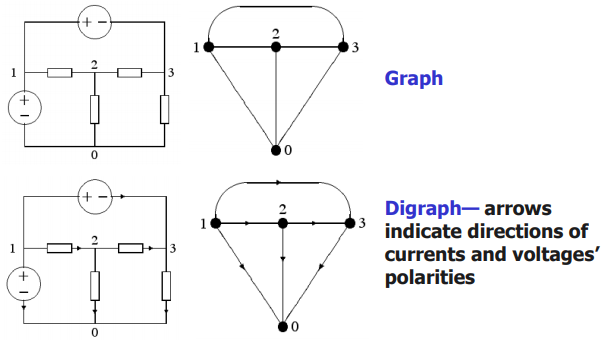
\includegraphics[width=5.5cm,height=5.5cm]{graphs.png}
    	\end{figure}
    \end{column}
\end{columns}
\end{frame}

\begin{frame}{Loop}
    \begin{columns}
        \begin{column}{.45\textwidth}
 		\begin{itemize}
			\item A loop is a set of branches of graph forming a closed path.
			\item Example: branches $\{a,c,d\}$, $\{b,d,e\}$ and $\{a,b,e,c\}$.		
		\end{itemize}
        \end{column}
		\begin{column}{.55\textwidth}
 		\begin{figure}[!ht]
  			\centering
    		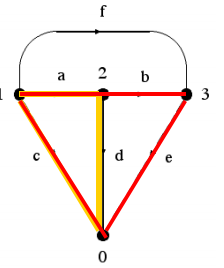
\includegraphics[width=0.6\textwidth]{loop.png}
   			 \caption[figure 3]{Braches and loops}
    		\label{fig:eg3}
    	\end{figure}
      	\end{column}
    \end{columns}
\end{frame}

\begin{frame}{Tree and co-tree}
\begin{itemize}
		\item A {\color{purple}tree} is a set of branches of a graph which contains no loop. 
		\item Thus, a tree is a maximal set of branches can be connected without forming a loop.
		\item After a tree is chosen, the remaining branches form a {\color{purple}co-tree}
\end{itemize}	
 		\begin{figure}[!ht]
  			\centering
    		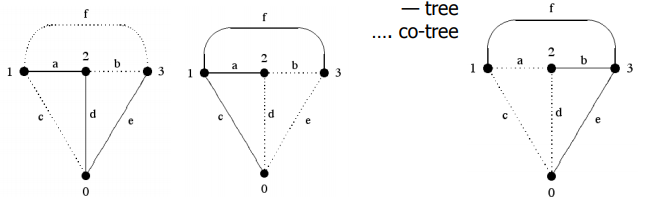
\includegraphics[width=0.6\textwidth]{tree1.png}
   			 \caption[figure 3]{Tree and co-tree}
    	%	\label{fig:eg3}
    	\end{figure}
\end{frame}

\section{Setting up Kirchhoff's equation}

\begin{frame}{A very simple example}
    \begin{columns}
        \begin{column}{.45\textwidth}
            \begin{table}[h!]
			%\begin{center}
	    	\caption{PSPICE netlist.}
	    	\label{tab:netlist}
	   		 \begin{tabular}{l|l|l|l} % <-- Alignments: 1st column left, 2nd middle and 3rd right, with vertical lines in between
	     	% \textbf{Value 1} & \textbf{Value 2} & \textbf{Value 3}\\
	     	% $\alpha$ & $\beta$ & $\gamma$ \\
	      		\hline
	      		I1 & 0 & 1 & 1Amp\\
	      		R2 & 1 & 0 & 1Ohm\\
	      		R3 & 1 & 2 & 1Ohm\\
	      		R4 & 2 & 0 & 1Ohm
	    	\end{tabular}
	  		%\end{center}
			\end{table}
        \end{column}
		\begin{column}{.75\textwidth}
         \begin{figure}[!ht]
  			\centering
    		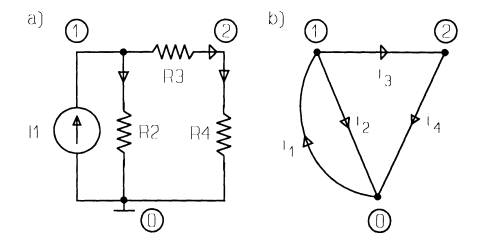
\includegraphics[width=0.7\textwidth]{circuitt.png}
   			 \caption[figure 4]{A simple circuit and its topology}
    		\label{fig:eg4}
    	 \end{figure}
      	\end{column}
    \end{columns}
\end{frame}

\begin{frame}{Kirchhoff's law again}
	\textbf{KVL}: At each loop or mesh,
	\begin{align*}
		\sum_{loop} V_k = 0
	\end{align*}
	\textbf{KCL}: At each node,
	\begin{align*}
		\sum I_{inflow} = \sum I_{outflow}
	\end{align*}

\end{frame}

\begin{frame}{A very simple example: KCL}
	The KCL equations w.r.t. node 1, 2 and 0 are
	\begin{align*}
		-I_1 + I_2 + I_3 &= 0\\
		-I_3 + I_4 + \,\, &= 0\\
		I_1 - I_2 - I_4 &=0
	\end{align*}
Linear dependency! $\Longrightarrow\,\,$, Reference node at which the KCL equations may be omitted.
\end{frame}

\begin{frame}{A very simple example: KCL}
Suppose we take node 0 as the reference node, so eliminate the 3rd equation, hence
\begin{align*}
	\begin{pmatrix} -1 & 1 & 1 & 0\\ 0 & 0 & -1 & 1 \end{pmatrix}
	\begin{pmatrix} I_1\\ I_2 \\I_3 \\I_4  \end{pmatrix} =0
\end{align*}
or simply
\begin{align*}
	A I = 0
\end{align*}
where $I$ is the vector of branch currents and $A$ is known as the {\color{purple}incidence matrix} containing only coefficients $0$ or $1$, $-1$.
\end{frame}

\begin{frame}{A very simple example: KVL}
\begin{itemize}
	\item Certain assembly of branches form loops (i.e. closed paths)
	\item In our last example, the loops are $\{I_1, R_2\}$, $\{I_1, R_3, R_4\}$ and $\{R_2, R_3, R_4\}$
	\item Conservation of energy: work done around a loop should be 0. Hence, the sum of voltages of branches constituting the loop must be 0.
In the similar vein, the KVL equations can be written as a compact matrix form as
\begin{align*}
	\begin{pmatrix} 1 & 1 & 0 & 0\\ 0 & -1 & 1 & 1 \end{pmatrix}
	\begin{pmatrix} v_1\\ v_2 \\v_3 \\v_4  \end{pmatrix} =0
\end{align*}

or simply
\begin{align*}
	B V = 0
\end{align*}
where $V$ is the vector of branch voltages and $B$ is known as the {\color{purple}loop matrix} containing only coefficients $0$ or $1$, $-1$.
\end{itemize}
\end{frame}

\begin{frame}{A very simple example: summary}
	By the superposition principle, the topological matrices $A$ and $B$ both contain the same full information on the assembly of branches.
\end{frame}

\begin{frame}{The formal procedure}
\begin{enumerate}
	\item Describe the circuit in a computer-readable format;
	\item Find a set of independent loops;
	\item For each loop, we associate a loop current;
	\item Use KVL to set up a system of $n$ equations, one for each independent loop;
	\item Solve the system of equations and thus find the values of the loop currents ($I$);
	\item Use the superposition principle to find the total current in each circuit branch.
\end{enumerate}
\end{frame}

\begin{frame}{A concrete example}

   \begin{columns}
        \begin{column}{.45\textwidth}
        \begin{itemize}
        	\item We show a set of independent loops with associated loop currents
        	\item Resistance are conventionally assumed to be ohms.
        	\item Voltage values are in volt.
        \end{itemize}

        \end{column}
		\begin{column}{.65\textwidth}
 	     \begin{figure}[!ht]
  			\centering
    		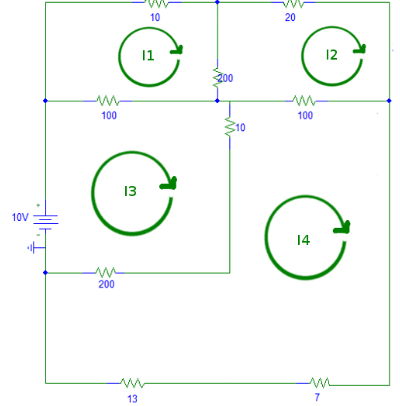
\includegraphics[width=0.7\textwidth]{concreteEg.png}
   			% \caption[figure 5]{Independent loops with associated loop currents}
    		\label{fig:eg5}
    	 \end{figure}
      	\end{column}
    \end{columns}
\end{frame}

\begin{frame}{A concrete example: setting up the Kirchhoff equations}
At each branch $b$, the total voltage drop $V^{(b)}$ across the branch is the sum of the voltage drop due to the loop currents $I_{l'}$ that traverse that branch:
\begin{align*}
	V^{(b)} &= \sum_{b\in l}\sum_{l'\in L_b} R^{(b)}I_{l'}
\end{align*}
So basically the inflow outflow relations,
\begin{align*}
	(10 + 200 + 100)I_1 - 200 I_2 - 100 I_3 + 0 I_4 &= 0\\
	-200 I_1 + (20 + 100 + 200) I_2 + 0 I_3 - 100 I_4 &= 0\\
	-100 I_1 + 0 I_2 + (100 + 10 + 200)I_3 - (200+10)I_4 &=10\\
	0 I_1 - 100 I_2 - (10+200) I_3 + (100 + 7 + 13 + 200 + 10) I_4 &= 0
\end{align*}
\end{frame}
%To solve one can simply use Gaussian elimination in any language of your favor.

\section{Setting up the Kirchhoff equations: an graph theoretic approach }

\subsection{Find spanning trees and fundamental set of circles (circuit base)}

\begin{frame}{Methods}
	\begin{itemize}
		\item  \href{https://dl.acm.org/doi/pdf/10.1145/363848.363861}{\beamergotobutton{Gotlieb and Corneil (1967)}}: Implementated by a Physicist Prof. Milotti's group, see \href{https://github.com/edymil/CircuitMath}{\beamergotobutton{CircuitMath}}.
		\item The above was further improved by \href{http://www.cs.kent.edu/~dragan/GraphAn/CycleBasis/p514-paton.pdf}{\beamergotobutton{Paton (1969)}}. The DFS search was used to construct cycle base: Computational very efficient!
		\item Further improved by \href{https://dl.acm.org/doi/pdf/10.1145/362814.362819}{\beamergotobutton{Tiernan (1970)}}. %Efficient but complicated. Fortunately this has been implemented in the Boost C++ libraries. See in particular the graph library . \hyperlink{https://www.boost.org/doc/libs/1_67_0/libs/graph/doc/graph_theory_review.html}{Boost::graph} provide a comprehensive range of headers including \href{https://www.boost.org/doc/libs/1_46_1/boost/graph/tiernan_all_cycles.hpp}{\beamergotobutton{Tiernan's}} efficient search algorithm in finding the fundamental cycles of the graph. 
	\end{itemize}
	In term of storage and speed, Paton and Tiernan are better. Moreover, Tiernan's algorithm has been written into the modern C++ numerics libraries like \href{https://www.boost.org/}{\beamergotobutton{Boost}}
\end{frame}

\begin{frame}{Method: \href{https://dl.acm.org/doi/pdf/10.1145/363848.363861}{Gotlieb and Corneil (1967)}}
	\textbf{Assumptions}
	\begin{itemize}
		\item Undirected graph is represented by its adjacency matrix $A=\{a_{ij}\}$ is
	\begin{align*}
		a_{ij} &= 
		\begin{cases}
			1 & \mbox{if $j$th node is connected with the $i$th node}\\
		%	-1& \mbox{if $j$th edge is incident into  the $i$th vertex}\\
			0& \mbox{if $j$th node is {\color{red}not} connected with the $i$th node}\\
		\end{cases}
	\end{align*}

	\item Graph is connected
	\item Each connected component can be separated
	\end{itemize}
	%\href{https://dl.acm.org/doi/pdf/10.1145/363848.363861}{\beamergotobutton{Gotlieb and Corneil (1967)}}
\end{frame}

\begin{frame}{Method: \href{https://dl.acm.org/doi/pdf/10.1145/363848.363861}{Gotlieb and Corneil (1967)}}
	\textbf{Key steps}
	\begin{itemize}
		\item Construct a set of disjoint trees by choosing some edges. 

		\begin{enumerate}
			\item The set of $n$ node is partitioned w.r.t. some chsen edges to form a set of disjoijnt trees with adjacency matrix $B$.
			\item For rach row $i$ of A, set $b_{ji}=b_{ij}=1$ if $a_{ij}$ is the first superdiagonal element of the $i$th row of $A$ to equal 1; otherwise set $b_{ji}=b_{ij}=0$.
		\end{enumerate}

	\item Divide the set of nodes of the graph into connected components w r.t. the edges chosen in step 1.
	\item Amalgamate the componets by adding appropriate edges to yield a spanning tree.
	\item Produce a set of fundamental cycles
	\end{itemize}
	%\href{https://dl.acm.org/doi/pdf/10.1145/363848.363861}{\beamergotobutton{Gotlieb and Corneil (1967)}}
\end{frame}
\begin{frame}{Method: \href{http://www.cs.kent.edu/~dragan/GraphAn/CycleBasis/p514-paton.pdf}{Paton (1969)}}
	This has been implemented by a computer scientist \href{https://www.codeproject.com/Articles/1158232/Enumerating-All-Cycles-in-an-Undirected-Graph}{Philipp Sch}. He demonstrated how in principle one can enumerate all cycles of a graph. However the method does not scale up well.
\end{frame}

\begin{frame}{Method: \href{https://dl.acm.org/doi/pdf/10.1145/362814.362819}{Tiernan (1970)}}
	A theoretically very eddifcient search algorithm that uses an exhaustive search to find all elementary circuits of a directed graph.  
	For more detail, one shall consult with 
	\begin{itemize}
		\item The official Boost Graph Library site : \href{https://www.boost.org/doc/libs/1_66_0/libs/graph/doc/quick_tour.html}{\beamergotobutton{boost::Graph}}
		\item Textbook: \href{}{\beamergotobutton{The Boost Graph library}}
		\item Uni-Resource: \href{http://cs.brown.edu/~jwicks/boost/libs/graph/doc/index.html}{\beamergotobutton{Brown}}
		\item Tutorial: \href{https://www.technical-recipes.com/2015/getting-started-with-the-boost-graph-library/}{\beamergotobutton{technical-recipes}}
	\end{itemize}
\end{frame}

%\subsection{Construct spanning tree}

%\subsection{Construct independent loops}

\subsection{Setting up the Kirchoff's law equations}

\begin{frame}{Circuit equations}
	Having found the independent loops, we can set up the system of equations like the one we show before and solve them. To fix idea,
	we consider mainly simple linear circuits. The solutions can be trivially attained using the LU decomposition method via some scientific software. 
	One choice is the routines \textbf{ludcmp} and \textbf{lubksb} in the Numerical Recipes C library
\end{frame}

\section{Solving the Kirchoff's law equations}


\begin{frame}{Branch currents and voltages}
	\begin{itemize}
		\item The solution of linear equation tields all the independent loop currents;
		\item From them, we can find the branch currents by summing over all the independent loop currents that traverse a given branch.
		\item By looping over all branches, one can construct a new matrix $I=\{i_{ik}\}$ where the element $i_{jk}$ stores the current in the branch that links the i-th node with the k-th node.
		\item Similarly, we calculate a voltage matrix $V=\{v_{jk}\}$, where the matrix elemet $v_{jk} = r_{jk}$, $i_{jk}$ stores the voltage drop in the branch that links the $j$th node with the $k$th node.
		\item Voltage are set by the power supplies w.r..t. a ground terminal: one can find the voltage of any node w.r.t. ground by following any path along the circuit that joins the node with the ground node and summing all the voltage drops.
		\item Finnaly, save the results on a file and save for further analysis
	\end{itemize}
\end{frame}

\begin{frame}{ Potential improvements}
	\begin{itemize}
		\item A comparison of graph-based method with the nodal method used in established programs such as SPICE
		\item Optimising circuit representation in the description file
		\item Deal with sparse matrix case, the program efficiency could be boosted with the use of sparse matrix code
		\item code could be cleaned up with C++, with introduction of linked lists represent loops and other graph structures
		\item Can be extended to handgle time-dependent voltage and currents, instead of the linear system we have seen, we can manipulate the corresponding DEs and use a DE solver
		\item Could be extended to include non-linear elements like semiconductor diades, transistors, etc, this would require the intro of a nonlinear equation solver
	\end{itemize}
\end{frame}

\begin{frame}{ Potential improvements}
	\begin{itemize}
		\item Can be implemented in Object-Oriented sense, utilise the efficient C++ library like Boost.
		\item Could work on a graphical interface both for input - by placing components in a special window - and for output - by automatically plotting output functions
		\item Could be used in the analysis of fluid flow - using the analogy between hydraulic and circuit networks.
	\end{itemize}
\end{frame}

\begin{frame}[fragile,shrink=30]{Future plan}
	Develop existing approach in modern C++. Make use of algorithm library and Boost.

% 	\lstset{language=C++}
% \begin{lstlisting}
\begin{minted}{c++}


#ifndef BOOST_GRAPH_CYCLE_HPP
#define BOOST_GRAPH_CYCLE_HPP

#include <vector>

#include <boost/config.hpp>
#include <boost/graph/graph_concepts.hpp>
#include <boost/graph/graph_traits.hpp>
#include <boost/graph/properties.hpp>

#include <boost/concept/detail/concept_def.hpp>
namespace boost {
    namespace concepts {
        BOOST_concept(CycleVisitor,(Visitor)(Path)(Graph))
        {
            BOOST_CONCEPT_USAGE(CycleVisitor)
            {
                vis.cycle(p, g);
            }
        private:
            Visitor vis;
            Graph g;
            Path p;
        };
    } /* namespace concepts */
using concepts::CycleVisitorConcept;
} /* namespace boost */
#include <boost/concept/detail/concept_undef.hpp>
\end{minted}
%\end{lstlisting}
\end{frame}



\end{document}